\section{Method}
\label{sec:method}

We present \textbf{AnomalyClaw}, a training-free visual anomaly detection (VAD) agent for cross-domain deployment. Rather than committing to one inference recipe, AnomalyClaw organises the design space around three orthogonal axes:

\begin{itemize}
    \item \textbf{Tools} --- action primitives that shape the input or produce side evidence: domain descriptor, reference retriever, hotspot cropper, component counter, knowledge lookup.
    \item \textbf{Experts} --- pretrained, non-parametric anomaly detectors that score the query against the normal reference set: SubspaceAD~\citep{subspacead2026}, DINOv2-giant patch-$k$-NN, DINOv2-giant global similarity.
    \item \textbf{Strategies} --- ways of combining the VLM with experts and tools: direct VLM, VLM--expert score fusion, proposer--advocate debate, hotspot interpret.
\end{itemize}

A lightweight \emph{router} picks a (tools, expert, strategy) triple per image. The router has two modes---a domain-descriptor rule set derived from the benchmark family taxonomy, and a calibration-driven argmax selector that uses 20 labelled items per domain---both of which are frozen before any test query is seen. The agent runs the selected strategy, records the trace, and returns a scalar anomaly score.

\paragraph{Framework vs.\ headline recipe.}
Sections~\ref{ssec:tools}--\ref{ssec:algorithm} describe our full
framework (router, strategy set, original calibration-argmax algorithm)
and produced the \emph{legacy} Findings~1--4 of \S\ref{sec:experiments}
(descriptor ablation, router-vs-fusion, etc.) on an earlier 12-domain
split. The paper's \emph{headline number} in Table~\ref{tab:main_results}
is produced by a different concrete instance of this framework, the
\textbf{AnomalyClaw ensemble agent} = refutation agent (\S\ref{ssec:refutation})
wrapped with a parallel independent Direct VLM call, described in
\S\ref{ssec:v10}. The calibration router from the design-exploration
phase is retained here for continuity with Findings~1--4; the ensemble
agent is the current system we benchmark in Table~\ref{tab:main_results}.

\begin{figure}[t]
    \centering
    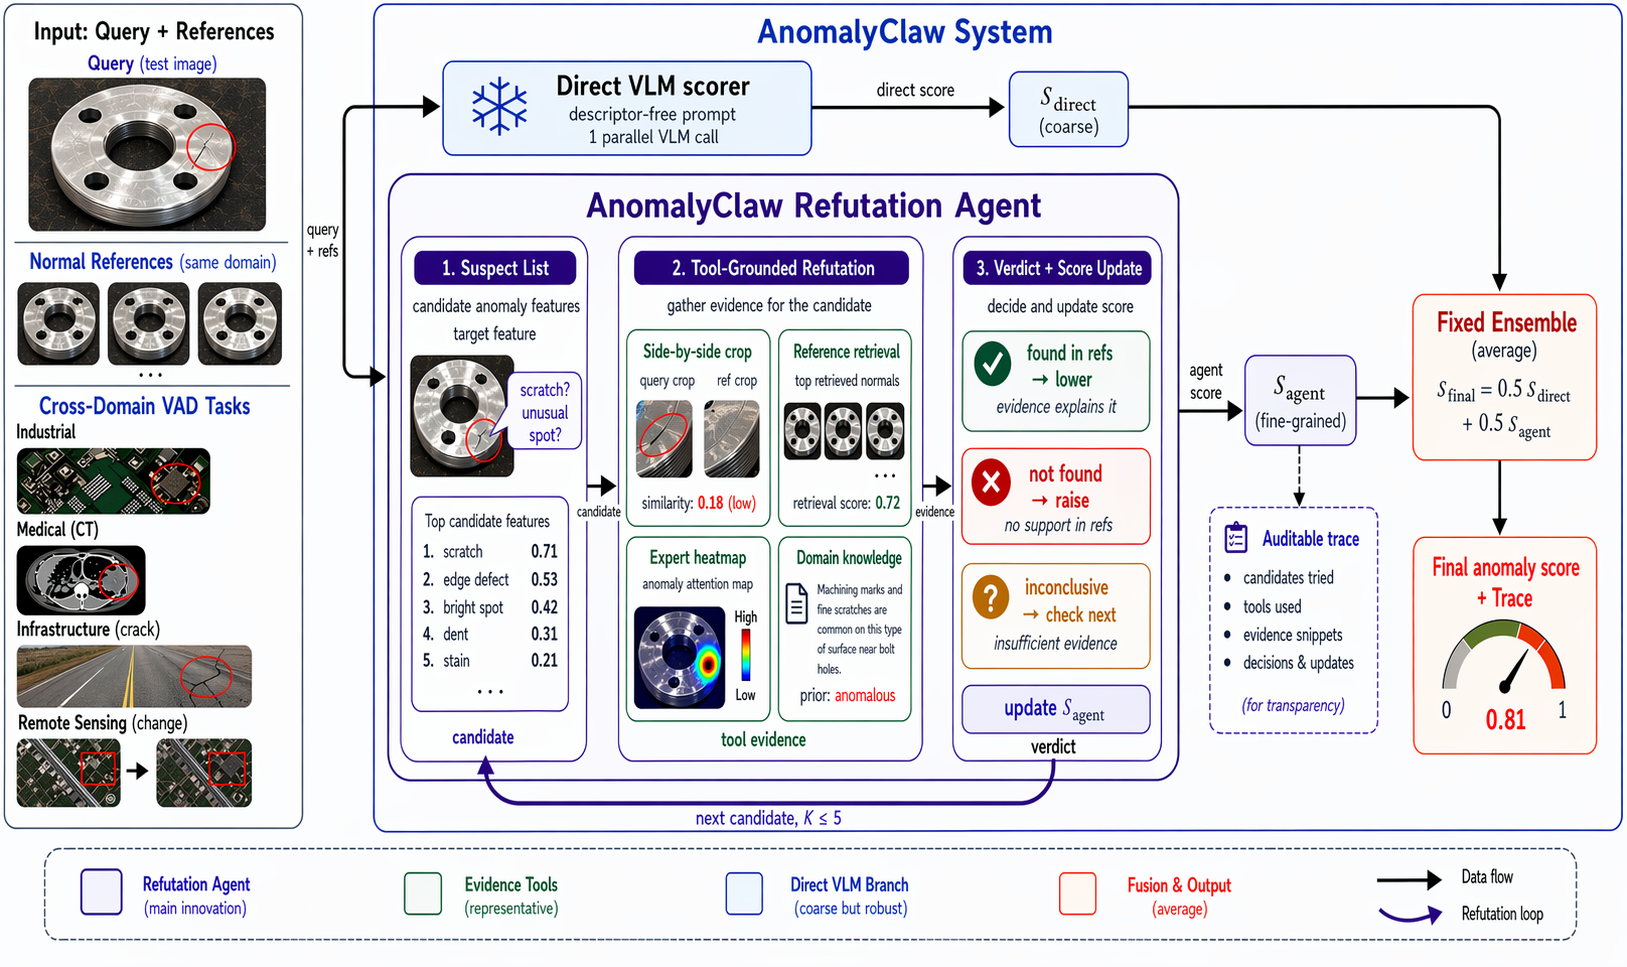
\includegraphics[width=\linewidth]{figures/fig_architecture_imagegen_hires.png}
    \caption{\textbf{AnomalyClaw architecture.} The headline system runs an independent Direct VLM scorer in parallel with a structured refutation agent. The agent proposes candidate anomaly features, uses frozen tool and expert evidence to refute them against normal references, and emits an auditable score. The final anomaly score is the fixed average of the Direct and agent scores, with no training or per-backbone tuning.}
    \label{fig:architecture}
\end{figure}

\subsection{Tool library}
\label{ssec:tools}
Each tool has a small, auditable contract; all tools are zero-VLM-call. The \texttt{domain\_descriptor} returns the task-anchored anomaly specification for the current domain (resolving generic-prior/task conflicts, e.g.\ D08 ``planned urbanisation IS the anomaly''). The \texttt{reference\_retriever} ranks the reference pool by DINOv2-CLS cosine similarity and returns the top-$k$. The \texttt{hotspot\_cropper} reads top-$k$ patch coordinates from an expert and crops the anomaly hotspot (used by the \emph{interpret} strategy). The \texttt{component\_counter} runs connected-component analysis on the expert hotspot map (logical anomalies). The \texttt{knowledge\_lookup} retrieves a domain keyword list for the VLM prompt (e.g.\ \emph{lesion, haemorrhage} for medical). Full tool signatures, I/O contracts, and implementations are in Appendix~\ref{app:tools}.

\subsection{Expert pool}
\label{ssec:experts}
The expert pool is intentionally diverse so the agent can pick the right inductive bias per domain. Two experts are pre-computed per item and cached; both produce a scalar anomaly score and (for SubspaceAD) the top-$k$ anomalous patches.
\begin{description}
    \item[\textbf{SubspaceAD}~\citep{subspacead2026}.] Training-free PCA reconstruction residual ($99\%$ EV) on DINOv2-giant patch tokens at $672{\times}672$ (layer mean $\{-12,\dots,-18\}$). Strong on industrial texture, retail packaging, logical anomalies (MVTec-LOCO), liver CT, brain MRI; weak on remote-sensing change and infrastructure cracks where the expected ``normal'' span is too narrow.
    \item[\textbf{AnomalyVFM}~\citep{anomalyvfm2025}.] Vision foundation model adapted via LoRA for zero-shot anomaly segmentation, with a convolutional decoder. We use the DINOv2 backbone variant; provides image-level score plus pixel mask. Complementary to SubspaceAD on infrastructure (calibration AUROC $0.72$ on D4 vs SubspaceAD's $0.50$) and on MVTec-LOCO logical anomalies where its synthetic-anomaly training data covers compositional defects.
\end{description}
A patch-$k$-NN side-channel on the same DINOv2-giant backbone provides $d_{\max}$, $\bar{d}_{\text{top5}}$, $d_{\text{base}}$, and a $48{\times}48$ hotspot map for the cropper tool; we did not use it as a primary expert in the reported results.

\subsection{Strategy set}
\label{ssec:strategies}
\begin{description}
    \item[\textbf{direct}.] One VLM call with the task-anchored descriptor and the first $k$ reference images. Cost: 1 VLM call.
    \item[\textbf{fusion(expert)}.] One VLM call (direct), then post-hoc blend with the chosen expert's score: $s = (1-w)\,s_{\mathrm{direct}} + w\,\sigma\!\big((s_{\mathrm{exp}}-m)/m\big)$, with $w$ frozen on calibration ($w{=}0.2$ as the global default; per-domain $w$ in Appendix~\ref{app:per_domain_w}). Both \emph{fusion(SubspaceAD)} and \emph{fusion(AnomalyVFM)} are first-class strategies.
    \item[\textbf{expert-only}.] No VLM call; the expert score is sigmoid-rescaled around the calibration median and used directly. Selected for domains where the calibration AUROC of the expert exceeds the best VLM-based strategy by $\ge 3$ pp (e.g.\ D7 GI endoscopy with SubspaceAD).
    \item[\textbf{zoom\_fusion}.] One VLM call, but the input is augmented with a high-resolution crop of the expert's hotspot region. Used when calibration shows the VLM benefits from a focused view.
    \item[\textbf{debate}.] Two VLM calls (proposer + advocate); rule-based aggregation (Appendix~\ref{app:debate}). Used when calibration shows VLM confidence is poorly calibrated on a domain.
\end{description}

\subsection{The agent: per-domain plan}
\label{ssec:router}
For each domain $d$, the agent selects a (\emph{strategy}, \emph{expert}) pair $\pi(d)$ from the joint catalogue. We use a \textbf{calibration argmax with a fusion-default}: the default plan is \emph{fusion(SubspaceAD)}, and we override only when the calibration AUROC of an alternative exceeds the default by at least $3$ pp (the ``override margin''). The 3-pp margin is itself frozen from a one-time sweep on a held-out backbone (GPT-5.4 calibration); we do \emph{not} retune it per backbone. Rationale: $20$ calibration items have a per-domain bootstrap noise floor of $\sim 2$ pp, so a margin slightly above the noise floor avoids over-fitting to small-sample noise.

The plan is computed once per (backbone, domain) pair and frozen before any test query. At inference time the agent looks up $\pi(d)$ and executes the strategy; no per-image router call is made. The final cost is the strategy's cost for that domain (Table~\ref{tab:main_results} reports an average of $0.92$ VLM calls/image on Qwen3.5).

\paragraph{Why this works.} Three single-strategy regimes map to different per-domain optima: \emph{fusion(SubspaceAD)} dominates texture / few-shot industrial, retail, brain MRI, liver CT, dermoscopy; \emph{direct} wins on semantic domains where the expert distorts the score (LEVIR change, SDNET infrastructure, road obstacle); \emph{expert-only} wins on domains where the expert is near-perfect (GI endoscopy with SubspaceAD AUROC $0.97$). A single fixed strategy cannot capture all three regimes.

\subsection{Algorithm}
\label{ssec:algorithm}

\begin{algorithm}[t]
\caption{\textsc{AnomalyClaw} agent inference.}
\label{alg:anomalyclaw}
\begin{algorithmic}[1]
\STATE \textbf{Input:} query $x$, references $\mathcal{R}$, domain $d$, descriptor $\phi_d$, frozen plan $\pi(d) = (S, E)$.
\STATE $s_E \leftarrow \mathrm{Expert}_E(x, \mathcal{R})$ \hfill\COMMENT{cached lookup; 0 VLM calls}
\IF{$S = \text{expert\_only}$}
    \STATE \textbf{return} $\sigma((s_E - m_E)/m_E)$ \hfill\COMMENT{0 VLM calls}
\ENDIF
\STATE $s_0 \leftarrow \mathrm{VLM}_{\mathrm{direct}}(x, \mathcal{R}, \phi_d)$ \hfill\COMMENT{1 VLM call}
\IF{$S = \text{direct}$}
    \STATE \textbf{return} $s_0$
\ELSIF{$S = \text{fusion}(E)$}
    \STATE \textbf{return} $(1 - w_d)\,s_0 + w_d\,\sigma((s_E - m_E)/m_E)$
\ELSIF{$S = \text{zoom\_fusion}(E)$}
    \STATE $c \leftarrow \mathrm{HotspotCropper}(x, \mathrm{Expert}_E.\text{patches})$
    \STATE $s_0 \leftarrow \mathrm{VLM}_{\mathrm{direct}}(x, \mathcal{R}, \phi_d, c)$ \hfill\COMMENT{1 VLM call with crop}
    \STATE \textbf{return} $(1 - w_d)\,s_0 + w_d\,\sigma((s_E - m_E)/m_E)$
\ELSIF{$S = \text{debate}$}
    \STATE \textbf{return} $\mathrm{Debate}(x, \mathcal{R}, \phi_d, s_0)$ \hfill\COMMENT{2 VLM calls}
\ENDIF
\end{algorithmic}
\end{algorithm}

\subsection{The ensemble agent (headline system)}
\label{ssec:v10}

The calibration router of \S\ref{ssec:router} is the framework that
produced Findings~1--4 on an earlier design-exploration split; the
paper's headline number in Table~\ref{tab:main_results} is produced by
a different concrete instance, the \textbf{AnomalyClaw ensemble agent}.
We describe the ensemble agent here to keep it clearly separated from
the router framework.

The ensemble agent wraps an autonomous multi-turn refutation agent
(described in \S\ref{ssec:refutation}) with an \emph{always-on parallel
Direct VLM call} running on the same backbone, and returns their
unweighted average. The two branches share no state: Direct sees the
query plus references under a descriptor-free task prompt and emits a
single anomaly score; the refutation agent sees the same inputs under a
refutation task preamble with a $K{=}5$ turn budget, and within those
turns can invoke any of $13$ tools (visual inspection, reference
understanding, structural analysis, cached expert probes,
semantic-knowledge lookup). Two of the $13$ tools make additional
VLM/LLM calls inside the tool body
(\texttt{tool\_reference\_profiler}, \texttt{tool\_domain\_knowledge});
the other eleven are zero-VLM-call data transformations or cached
lookups. The refutation component therefore issues between $1$ and $5$
VLM calls per query (average $\approx 1.8$ across the three backbones
on CrossDomainVAD-12) plus the single parallel Direct call. The final
ensemble score is
\[
  s_{\mathrm{final}} \;=\; 0.5 \cdot s_{\mathrm{Direct}} + 0.5 \cdot s_{\mathrm{agent}},
\]
with $\alpha{=}0.5$ fixed a priori (no dev tuning). Direct and the
refutation agent run concurrently on the same backbone API session, so
per-item wall-time is $\max(\text{Direct},\,\text{agent})$ rather than
the sum.

The \textbf{always-on} design is the load-bearing choice. An
alternative architecture would run the agent alone and skip the Direct
branch whenever the agent is expected to outperform Direct. We find
that on Qwen3.5-VL-27B the agent alone is significantly \emph{worse}
than Direct ($-4.46$~pp macro AUROC on CrossDomainVAD-12 test, 95\%
CI $[-7.61,-1.55]$, $P{=}0.001$); yet the always-on ensemble still
produces a positive macro gain over Direct ($+1.69$~pp, $P{=}0.971$).
The same architecture gives larger gains when the agent is individually
strong (GPT-5.4: agent-alone $+3.64$~pp vs Direct, ensemble
$+4.01$~pp) and when both branches contribute (SeedVL: agent-alone
$+3.68$, ensemble $+5.99$). A pure agent pipeline silently loses on
backbones where the agent is the weaker estimator; the always-on Direct
branch makes the ensemble robust to that failure mode without
per-backbone tuning.

\subsection{Refutation agent}
\label{ssec:refutation}

The refutation agent is a structured deliberation protocol that
directly targets two failure modes observed in unstructured ReAct
agents: (i) \emph{coarse rank grid}---the VLM emits scores drawn from a
small set of unique values, which limits ranking resolution and caps
AUROC gains; (ii) \emph{confirmation bias}---tool calls tend to support
the VLM's working hypothesis rather than test it. The task-aware
preamble allows the same runner to handle anomaly scoring, MCQ choice,
and open-ended answers from a single trajectory (\S\ref{ssec:mmad_v9});
for Table~\ref{tab:main_results} only the anomaly-scoring mode is
exercised.

\paragraph{Protocol.}
The refutation agent replaces the free-form ``call any tool, update
score'' pattern with a structured three-phase schema:
\begin{enumerate}
    \item \textbf{Suspect list (turn 1, no tool).} The VLM outputs an \texttt{initial\_score}, a list of up to three \texttt{candidate\_features}~$=\{(\text{name}_i, \text{location\_hint}_i, \text{looks\_defect\_like}_i)\}$ and a \texttt{refutation\_target} index~$t^*$ into that list. The prompt fixes the default: if \texttt{candidate\_features} is empty and \texttt{initial\_score}~$<0.3$, the agent finalises at~$0.05$ without calling a tool.
    \item \textbf{Targeted refutation (turn 2+).} The agent calls a refutation tool whose output is about \emph{whether the feature at $t^*$ appears in any reference}. \texttt{tool\_side\_by\_side} crops query and four refs at the same bbox; \texttt{tool\_reference\_profiler} returns a structured normal-baseline profile (object, colors, allowed variations); \texttt{tool\_reference\_retriever} fetches top-$k$ similar normals. Each output is paired with an explicit \texttt{interpretation} field containing a disconfirm clause, e.g.\ ``the bright region in the composite also appears in ref 2 at the same position.''
    \item \textbf{Verdict and update.} The VLM emits \texttt{refutation\_verdict} $\in \{\text{found\_in\_ref}, \text{not\_found}, \text{inconclusive}\}$, removes refuted features from \texttt{remaining\_candidate\_features}, and outputs \texttt{updated\_score}. If the remaining list is empty the score is forced into $[0.05, 0.20]$; if at least one feature survives the score is in $[0.40, 0.95]$ proportional to its defect-likeness. Remaining features are checked in subsequent turns until the $K{=}5$ budget is exhausted.
\end{enumerate}

\paragraph{Why this counters confirmation bias.}
In a free-form ReAct agent a tool is invoked to \emph{support} the VLM's working hypothesis and the system accumulates supporting observations. In the refutation protocol, every tool output has exactly one legitimate use---retiring a candidate feature---so the protocol is naturally biased toward ruling anomalies \emph{out}. The structured output (\texttt{candidate\_features}, per-turn \texttt{refutation\_verdict}, \texttt{remaining\_candidate\_features}) gives a reviewer an auditable trace.

\paragraph{Ensembling with Direct.}
The refutation agent alone does not uniformly beat Direct across backbones (Table~\ref{tab:main_results}: $+3.64$/$+3.68$/$-4.46$ pp on GPT-5.4/SeedVL/Qwen3.5). We therefore always average the agent output with an \emph{independent} parallel Direct call from the same VLM backbone:
\[
  s_{\mathrm{final}} \;=\; 0.5 \cdot s_{\mathrm{Direct}} + 0.5 \cdot s_{\mathrm{agent}},
\]
with $\alpha{=}0.5$ fixed a priori. This always-on design (described in \S\ref{ssec:v10}) produces the ensemble gains in Table~\ref{tab:main_results}: $+4.01$ pp on GPT-5.4 and $+5.99$ pp on SeedVL (both significant at $95\%$, $P{=}1.000$), and $+1.69$ pp on Qwen3.5-VL-27B (positive-in-mean, $95\%$ CI $[-0.08,+3.51]$ just touches zero) --- including on Qwen3.5, where the agent alone is individually worse than Direct.

\paragraph{Rank-granularity mechanism.}
Section~\ref{ssec:score_diversity} isolates the causal driver of the ensemble gain via rank-preserving and rank-collapsing transformations of the agent's scores. On an earlier design-exploration split on Qwen3.5 we measured Direct at $11$ unique scores on the test set and a free-form JSON agent at $49$; averaging the two fills in the rank ties inside Direct's coarse bimodal clusters with real signal. Transformations that preserve the agent's unique-value grid retain the full gain; a median-split binarisation that collapses the grid to $2$ values cuts the gain in half. Section~\ref{ssec:score_diversity} retains that analysis as evidence for the rank-granularity mechanism; the mechanism is agent-family agnostic, although the absolute unique-value count differs by runner.

\subsection{Design principles}
\label{ssec:principles}
\begin{itemize}
    \item \textbf{No training.} All VLMs and experts are frozen. SubspaceAD's PCA is a closed-form fit on reference features; patch-$k$-NN is a direct distance computation.
    \item \textbf{No per-domain code.} The only per-domain artefact is the descriptor $\phi_d$ (one sentence) plus a family tag used by the descriptor router; both are written once.
    \item \textbf{Bounded call budget.} The ensemble agent issues 1 Direct call plus $1$--$5$ refutation agent turns per item; the average across CrossDomainVAD-12 is $\approx 1.0 + 1.8 = 2.8$ VLM calls/item with the two branches running concurrently ($\sim 1.8$ wall-time calls due to parallel execution).
    \item \textbf{Auditable decisions.} Every output is accompanied by a trace listing the tools invoked, the expert selected, the chosen strategy, and (when applicable) the VLM's two-call evidence. Appendix~\ref{app:trace} shows a full trace example.
\end{itemize}
